
\section{Introducción}
Las ecuaciones diferenciales de orden superior tienen aplicaciones fundamentales en la modelización de sistemas físicos, biológicos, económicos y de ingeniería. Este capítulo explora diversas aplicaciones prácticas en las que se emplean ecuaciones diferenciales de segundo y mayor orden para describir fenómenos del mundo real. 

Cada problema abordado incluirá una descripción detallada, la formulación matemática del modelo, su resolución y una interpretación gráfica de los resultados.

\section{Oscilaciones Mecánicas: Masa-Resorte-Amortiguador}
Un modelo clásico en la mecánica es el sistema masa-resorte-amortiguador, que describe el movimiento de una masa sujeta a un resorte y sometida a una fuerza de amortiguamiento.

\subsection*{Ejemplo 1: Movimiento de un Oscilador Amortiguado}
Se tiene un bloque de masa \( m = 5 \) kg unido a un resorte con constante \( k = 100 \) N/m y sometido a una fuerza de amortiguamiento proporcional a la velocidad con coeficiente \( c = 10 \) Ns/m. Se suelta desde una posición de 0.2 m con velocidad inicial cero. Encontrar su movimiento y graficar la solución.

\textbf{Ecuación de Movimiento:}

\begin{equation}
m y'' + c y' + k y = 0
\end{equation}

Sustituyendo los valores:

\begin{equation}
5 y'' + 10 y' + 100 y = 0
\end{equation}

La ecuación característica es:

\begin{equation}
5r^2 + 10r + 100 = 0
\end{equation}

Resolviendo para \( r \), obtenemos raíces complejas \( r = -1 \pm i \sqrt{19} \), lo que nos da la solución:

\begin{equation}
y(t) = e^{-t} \left( C_1 \cos (\sqrt{19}t) + C_2 \sin (\sqrt{19}t) \right)
\end{equation}

Usando las condiciones iniciales, determinamos \( C_1 \) y \( C_2 \). Finalmente, la solución se grafica para visualizar la oscilación amortiguada.

\begin{figure}[H]
    \centering
    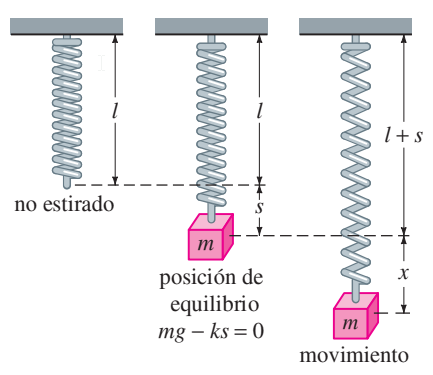
\includegraphics[width=0.5\linewidth]{images/Modelado 06.png}
    \caption{Movimiento amortiguado de la masa}
    \label{fig:enter-label}
\end{figure}

\subsection*{Ejercicio para Resolver}
Un oscilador con \( m = 3 \) kg, \( k = 50 \) N/m y \( c = 8 \) Ns/m se desplaza desde una posición inicial de 0.1 m con velocidad de 0.2 m/s. Determine la ecuación de su movimiento y grafique su comportamiento.

\section{Vibraciones en Circuitos Eléctricos}
Un circuito \( RLC \) en serie se modela con la ecuación:

\begin{equation}
L \frac{d^2q}{dt^2} + R \frac{dq}{dt} + \frac{1}{C} q = 0
\end{equation}

\subsection*{Ejemplo 2: Descarga de un Circuito RLC}
Se tiene un circuito con \( L = 2 \) H, \( R = 4 \) \( \Omega \) y \( C = 0.5 \) F. La carga inicial es de 10 C y la corriente inicial es 0. Determinar la ecuación de descarga.

La ecuación característica es:

\begin{equation}
2r^2 + 4r + 2 = 0
\end{equation}

Resolviendo para \( r \), obtenemos raíces reales e iguales, por lo que la solución es:

\begin{equation}
q(t) = (C_1 + C_2 t) e^{-t}
\end{equation}

\begin{figure}[H]
    \centering
    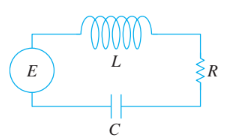
\includegraphics[width=0.5\linewidth]{images/Modelado 07.png}
    \caption{Disminución de la carga en el circuito RLC.}
    \label{fig:enter-label}
\end{figure}


\subsection*{Ejercicio para Resolver}
Un circuito RLC tiene \( L = 1.5 \) H, \( R = 3 \) \( \Omega \) y \( C = 0.4 \) F. La carga inicial es 5 C y la corriente inicial es 0. Determine la ecuación de descarga y grafique la variación de la carga con el tiempo.

\section{Flexión de Vigas en Ingeniería}
La ecuación de flexión de una viga bajo carga se modela mediante:

\begin{equation}
EI \frac{d^4 y}{dx^4} = w(x)
\end{equation}

\subsection*{Ejemplo 3: Deflexión de una Viga bajo Carga Uniforme}
Una viga simplemente apoyada de longitud \( L = 10 \) m soporta una carga uniforme de 500 N/m. Si \( EI = 2 \times 10^6 \) Nm\(^2\), determinar la deflexión.

Resolviendo la ecuación diferencial con las condiciones de frontera:

\begin{equation}
y(x) = \frac{w}{24EI} x^4 - \frac{wL}{12EI} x^3 + C_1 x + C_2
\end{equation}

La deflexión máxima ocurre en el centro de la viga.


\begin{figure}[H]
    \centering
    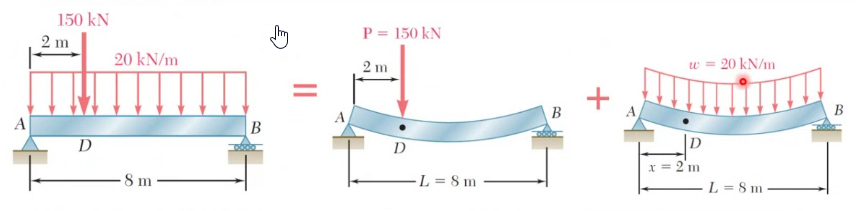
\includegraphics[width=0.5\linewidth]{images/Modelado 08.png}
    \caption{Curvatura de la viga bajo carga uniforme.}
    \label{fig:enter-label}
\end{figure}

\subsection*{Ejercicio para Resolver}
Una viga de 8 m de largo soporta una carga distribuida de 300 N/m y tiene \( EI = 1.5 \times 10^6 \) Nm\(^2\). Encuentre la ecuación de la deflexión y grafique la forma de la viga.

\section{Conclusión}
Las ecuaciones diferenciales de orden superior proporcionan herramientas esenciales para modelar sistemas dinámicos en ingeniería y ciencias aplicadas. La interpretación gráfica de las soluciones nos permite analizar el comportamiento de los sistemas y predecir su evolución en el tiempo.

